% Some notation taken from 
% https://cs230.stanford.edu/files/Notation.pdf

% On variables, parameters, and arguments
% https://math.stackexchange.com/questions/2113138/what-is-the-difference-between-variable-argument-and-parameter

\documentclass{article}
\usepackage[sorting=none]{biblatex}
\addbibresource{sources.bib}

%Graphics: https://www.overleaf.com/learn/latex/Inserting_Images
\usepackage{graphicx}
\graphicspath{{figures/}}

% https://tex.stackexchange.com/questions/2651/should-i-use-center-or-centering-for-figures-and-tables
\makeatletter
\g@addto@macro\@floatboxreset\centering
\makeatother

% https://tex.stackexchange.com/questions/268766/curly-braces-in-math-mode
\usepackage{mathtools}
\DeclarePairedDelimiter\set\{\}

% https://github.com/battlesnake/neural
% \usepackage{neuralnetwork}

\usepackage{amsmath}

% Titular information
% https://en.wikibooks.org/wiki/LaTeX/Title_Creation
\title{
	An Undergraduate's Explanation of the Multilayer Perceptron: 
	Mathematical Concepts and a Python3 Implementation}
\date{2022 \\ January}
\author{Jared Frazier\thanks{Department of Computer Science (2021-2022), 
Middle Tennessee State University} \thanks{Not endorsed by or affiliated with any of the 
authors or entities associated with references}}
\begin{document}
\maketitle

\section{Preamble}
\quad The purpose of the present document is to explain and implement the major mathematical
constructs/concepts behind feedforward neural networks, specifically the multilayer perceptron.
This includes the layers that compose such networks, the cost (aka loss, error, or objective) function
and activation functions, the forward pass through the network,
the computation of gradients via backpropagation (a concept that is often "handwaved" to the extreme
or explained in so much detail as to be utterly confusing--at least in the author's experience),
and the update of model parameters via mini-batch stochastic gradient descent.
If the ideas such as \textit{layer} and \textit{backpropagation} are entirely unfamiliar
to you, then the author encourages you to visit 3Blue1Brown's Deep Learning YouTube Series \cite{3Blue1BrownWhatIsANN2017}
and peruse the first few chapters of texts such as \textit{Deep Learning} (free, online) \cite{Goodfellow2016},
\textit{Neural Networks and Deep Learning} (free, online) \cite{Nielsen2015},
\textit{Hands-on Machine Learning with Scikit-Learn, TensorFlow and Keras 2ed} (buy) \cite{Geron2020},
and/or \textit{Deep Learning with Python 2ed} (buy) \cite{Chollet2021}. The present document
is not intended to be a comprehensive overview of neural networks nor an extremely
in-depth mathematical treatise but rather a document that highlights certain concepts that the
author found confusing or ambiguous when he was learning about neural networks
(particularly regarding the backpropagation algorithm).

The format of explanations in the present document will essentially alternate between mathematics
and concrete implementations using the Python3 programming language with
the NumPy library. Note that the implementations here
are not intended to be optimal. If you would like optimal implementations, the author
encourages you to use a machine learning API such as TensorFlow or PyTorch, the tutorials
for which will abstract and make easily usable many of the concepts elucidated in
the present document.

\section{Introduction}

\quad The neural network (function approximator) is just a chain of geometric transformations (functions)
each parametrized by a weight matrix $W \in \mathcal{R}^{n_h \times n_x}$ and
a bias vector $b \in \mathcal{R}^{n_h}$ on the input vector $x \in \mathcal{R}^{n_x}$.
The geometric transformations of the neural network are encapsulated by connecting
layers (e.g., dense/fully connected layers) together. A neural network has $L$ total
layers and the current layer $l$ receives the output from the previous layer $(l-1)$.
Note that $n_x$ is the number of features (or independent variables) in the input
and $n_h$ is the number of hidden units in the current layer. The following subsections will
breifly elucidate the claims in of the first setnence of this section and the
corresponding notation.

\subsection{Parametrized Functions}

The author assumes you know what a function is; however, the term \textit{parametrized}
is one that appears often in deep learning literature and should be well-understood by the student.
Consider a generic quadratic function \cite{MathSEVarsParamsArgs2015} as
% Quadratic function
\begin{equation}
	f(x) = ax^{2} + bx + c
\end{equation}
The \textit{variable} $x$ is an \textit{argument} to the function $f$ that has
\textit{parameters} $a$, $b$, and $c$. The parameters determine the behavior of
the function (e.g., the steepness of slope, intercepts, shape, etc.) while the
variable can take on some range of values. When a variable that takes on a particular
value is passed as an argument to the function with defined parameters, the result
is some other value $y$ if $y = f(x)$. This explanation of a function
should not be anything new; however, the \textit{parameters} are quantities
of particular interest for neural networks since the parameters are the quantities
that are \textit{learned} by the neural network over time. What it means to learn
parameters will be explaned later.

A neural network can be denoted as a function $h$ with parameters $W$
and $b$ of a variable $x$. This statement can be compactly written as
$h_{W, b}(x)$. The subscript with $W$ and $b$
means that the weights $W$ and biases $b$ are parameters of the neural network $h$.
The claim that a neural network is a chain of functions is useful later during
the updating of the parameters of the network. But to briefly illustrate the idea
of chaining functions, the generic quadratic function in Equation 1 is decomposed
into units called \textit{atomic functions}.
\begin{align}
	g_{a}(x)     & = ax^{2}                  \\
	u_{b}(x)     & = bx                      \\
	f_{a,b,c}(x) & = g_{a}(x) + u_{b}(x) + c
\end{align}
Decomposing functions into their constituent atomic functions is useful
for applying rules of calculus--the basis of parameter learning via
the backpropagation algorithm illustrated later.

\subsection{Operand Types}

The input $x$ is not a single value as is conceived in the elementary
formulations described above. Rather, the input $x$ is a list of
values referred to as a \textit{column vector}. Each element of the vector
is the value a particular feature, or independent variable, could take on.
The shape of the vector $x$ is important to understand since the functions and operations
performed by the neural network (dot product, Hadamard product, addition, etc.)
restrict their vector/matrix operands to particular shapes. When using the term
\textit{vector}, the author is always referring to a \textit{column vector}
unless otherwise specified. Also, note that $x \in \mathcal{R}^{n_x}$ indicates
that $x$ is a vector with $n_x$ elements and the $j^{th}$ is a real number.
For example, the below vector $x$ is shown and a common vector operation
known as transposition (converts a \textit{column vector} to a
\textit{row vector} and is denoted with a superscript of $\top$) is also shown.
\begin{align}
	x & = \begin{bmatrix}
		x_{1}  \\
		x_{2}  \\
		x_{3}  \\
		\vdots \\
		x_{(n_x)}
	\end{bmatrix}
	=
	\begin{bmatrix}
		x_{0}  \\
		x_{1}  \\
		x_{2}  \\
		\vdots \\
		x_{(n_{x}-1)}
	\end{bmatrix}
	=
	\begin{bmatrix}
		x_{0} & x_{1} & x_{2} & \cdots & x_{(n_{x}-1)}
	\end{bmatrix}^\top
\end{align}

Many programming languages assign the first element of a vector the index
0; this notation is shown above in addition to the more standard
mathematical notation where the first element begins with the index 1.
For the remainder of this document, the author will use the index 0 assumption
since the author's implementation of the the neural network will use the Python
programming language. If you wish to implement the same algorithms in a language
such as R or Wolfram Mathematica, be wary of this index discrepancy.
Consequently, with index beginning at 0, the last index of a vector with
$n_x$ elements will be $(n_x - 1)$... and woe is the programmer who commits an
off-by-one error.

Lastly, a matrix $W$ represents the weight of edges between the $k^{th}$
input neuron of $n_x$ total input neurons (i.e., neurons in the previous layer)
and the $j^{th}$ hidden neuron of $n_h^{l}$ total hidden neurons.
A weight matrix looks similar to the vector, except rather than having a single
column, a matrix has a rows and columns--looking like a table. Vectors can
be referred to as rank-1 tensors, matrices as rank-2 tensors, so and so forth
for multiple index "lists" in higher dimensions. A sample weight matrix
$W \in \mathcal{R}^{n_h \times n_x}$ is
shown below.

\begin{align}
	\begin{bmatrix}
		W_{00}         & W_{01}         & W_{02}         & \cdots & W_{0(n_{x}-1)}         \\
		\vdots         & \vdots         & \vdots         & \vdots & \vdots                 \\
		W_{(n_{h}-1)0} & W_{(n_{h}-1)1} & W_{(n_{h}-1)2} & \cdots & W_{(n_{h}-1)(n_{x}-1)}
	\end{bmatrix}
\end{align}

\section{The Multilayer Perceptron}
\quad Here the author defines the operations that occur for a multilayer perceptron (MLP).
Note that the MLP can sometimes refer to any class of feedforward
neural network, that is a network that applies affine transformations and
activation functions to input from a previous layer in the network.

\subsection{The Dense/Fully Connected Layer}
The affine transformation, which is the most fundamental transformation
of the densely/fully connected layers that exist in the MLP, yields
a weighted input element $z_j^{l} = W_{jk}^{l} a_{k}^{l-1} + b_{j}^{l}$. Here,
the activation $a_k^{l-1}$ denotes the activation of the $k^{th}$ neuron of the
previous layer $(l-1)$. Importantly, the input layer has no activation function $\phi$
associated with it, so the activation vector $a^{0}$ equal the input vector $x$.
Moreover, the inner dimensions of the matrix product
$Wx$ match, that is the subscripts $k$ are "adjacent" to one another. While you may
observe that the activation vector $a \in \mathcal{R}^{n_a}$ is clearly not a matrix,
numerical libraries will often treat a vector $v \in \mathcal{R}^{n_v}$ as equivalent
to a matrix with a single column (i.e., $V \in \mathcal{R}^{n_v \times 1}$) for
the purposes of performing fast matrix-matrix calculations.

Until now the discussion of the MLP has been entirely in abstract mathematical
notation, so now a visual of a single layer (meaning single hidden layer)
MLP is shown. The activation function $\phi$ is vectorized, meaning it
applies to each element of a vector, matrix, or rank-n tensor. The weighted input
vector $z^{l} = \set{ z_{j}^{l} }_{j=0}^{n_{h} - 1}$, meaning there is an element
of the weighted input vector for the $j^{th}$ neuron in a layer. The number of
neurons in a hidden layer (or output layer for that matter) $n_h$ does not have
to be constant, and this is shown in the figure below where the output layer
has only a single neuron while the hidden layer has three neurons.

% Multilayer perceptron figure
\begin{figure}[h]
	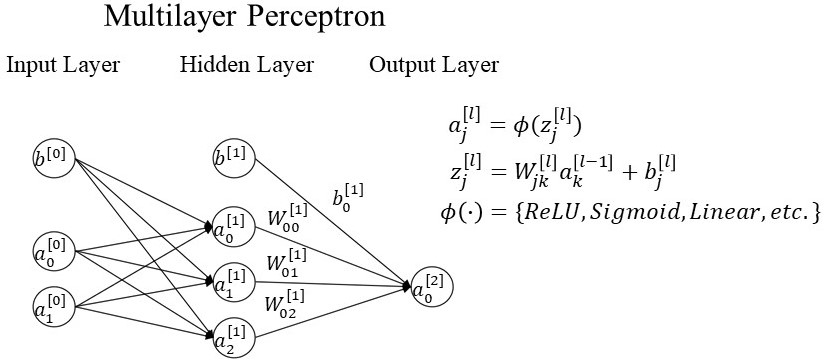
\includegraphics[scale=0.60]{mlp_larger_font_croppped.jpg}
\end{figure}

% Multilayer percetpron with useneuralnetwork pkg
% \begin{align}
% 	\begin{neuralnetwork}[height=3, layertitleheight=5.0em]
% 		\newcommand{\x}[2]{$a^{0}_#2$}
% 		\newcommand{\hfirst}[2]{\small $a^{(1)}_#2$}
% 		\newcommand{\y}[2]{$a^{2}_#2$}
% 		\inputlayer[count=2, bias=false, title=Input Layer 0, text=\x, nodeclass={input neuron}]
% 		\hiddenlayer[count=3, bias=false, title=Hidden Layer 1, text=\hfirst, nodeclass={hidden neuron}] \linklayers
% 		\outputlayer[count=1, title=Output Layer 2, text=\y, nodeclass={output neuron}] \linklayers
% 	\end{neuralnetwork}
% \end{align}

% Neural Network Definition
\subsection{Single Hidden Layer Neural Network}
\begin{equation}
	\begin{aligned}
		NeuralNet_{\theta}(X) & =
		\sigma(ReLU(XW^{[1]}
		+ {b}^{[1]})W^{[2]} + {b}^{[2]})                                                                  \\
		                      & = \sigma(g(ReLU(w(X))))                                                   \\
		A^{L}                 & = NeuralNet_{\theta}(X) & \text{Activation matrix $A$ for last layer $L$}
	\end{aligned}
\end{equation}

where $\sigma$, $ReLU$, $g$, and $w$ are defined as follows:

\begin{equation}
	\begin{aligned}
		\sigma(t)           & = \frac{1}{1 + e^{-t}}                                                         \\
		ReLU(t)             & = max(0, t)                                                                    \\
		g_{\theta^{[2]}}(A) & = AW^{[2]} + {b}^{[2]}                                                         \\
		w_{\theta^{[1]}}(A) & = AW^{[1]} + {b}^{[1]}                                                         \\
		u_{\theta^{[l]}}(A) & = AW^{[l]} + b^{[l]}   & \text{General form of $g$ and $w$ for $l^{th}$ layer}
	\end{aligned}
\end{equation}

\subsection{Neural Network Prediction (Forward Pass)}
% Forward Pass
\begin{align}
	\hat{y} & \gets NeuralNet_\theta(X)
\end{align}

% Loss function
\subsection{Mean Squared Error Loss Function}
\begin{equation}
	\begin{aligned}
		\mathcal{L}_\theta(X) & =
		\frac{1}{N} \sum_{i=1}^{N}{ (\hat{y}^{(i)} - y^{(i)} )^{2}}                                                                                                            \\
		                      & = \frac{1}{N} \sum_{i=1}^{N}{(a^{(i)} + y^{(i)})^{2}} & \text{$a^{(i)}$ is the activation vector of the last layer $L$ for the $i^{th}$ input}
	\end{aligned}
\end{equation}

\subsection{Gradient Update}
% Weight updates
\begin{align}
	\theta_i & \gets \theta_i - \eta (\nabla_\theta \mathcal{L}_{\theta}(\hat{y}, y))
\end{align}

\printbibliography

\end{document}